\begin{figure}[H]
	\centering
	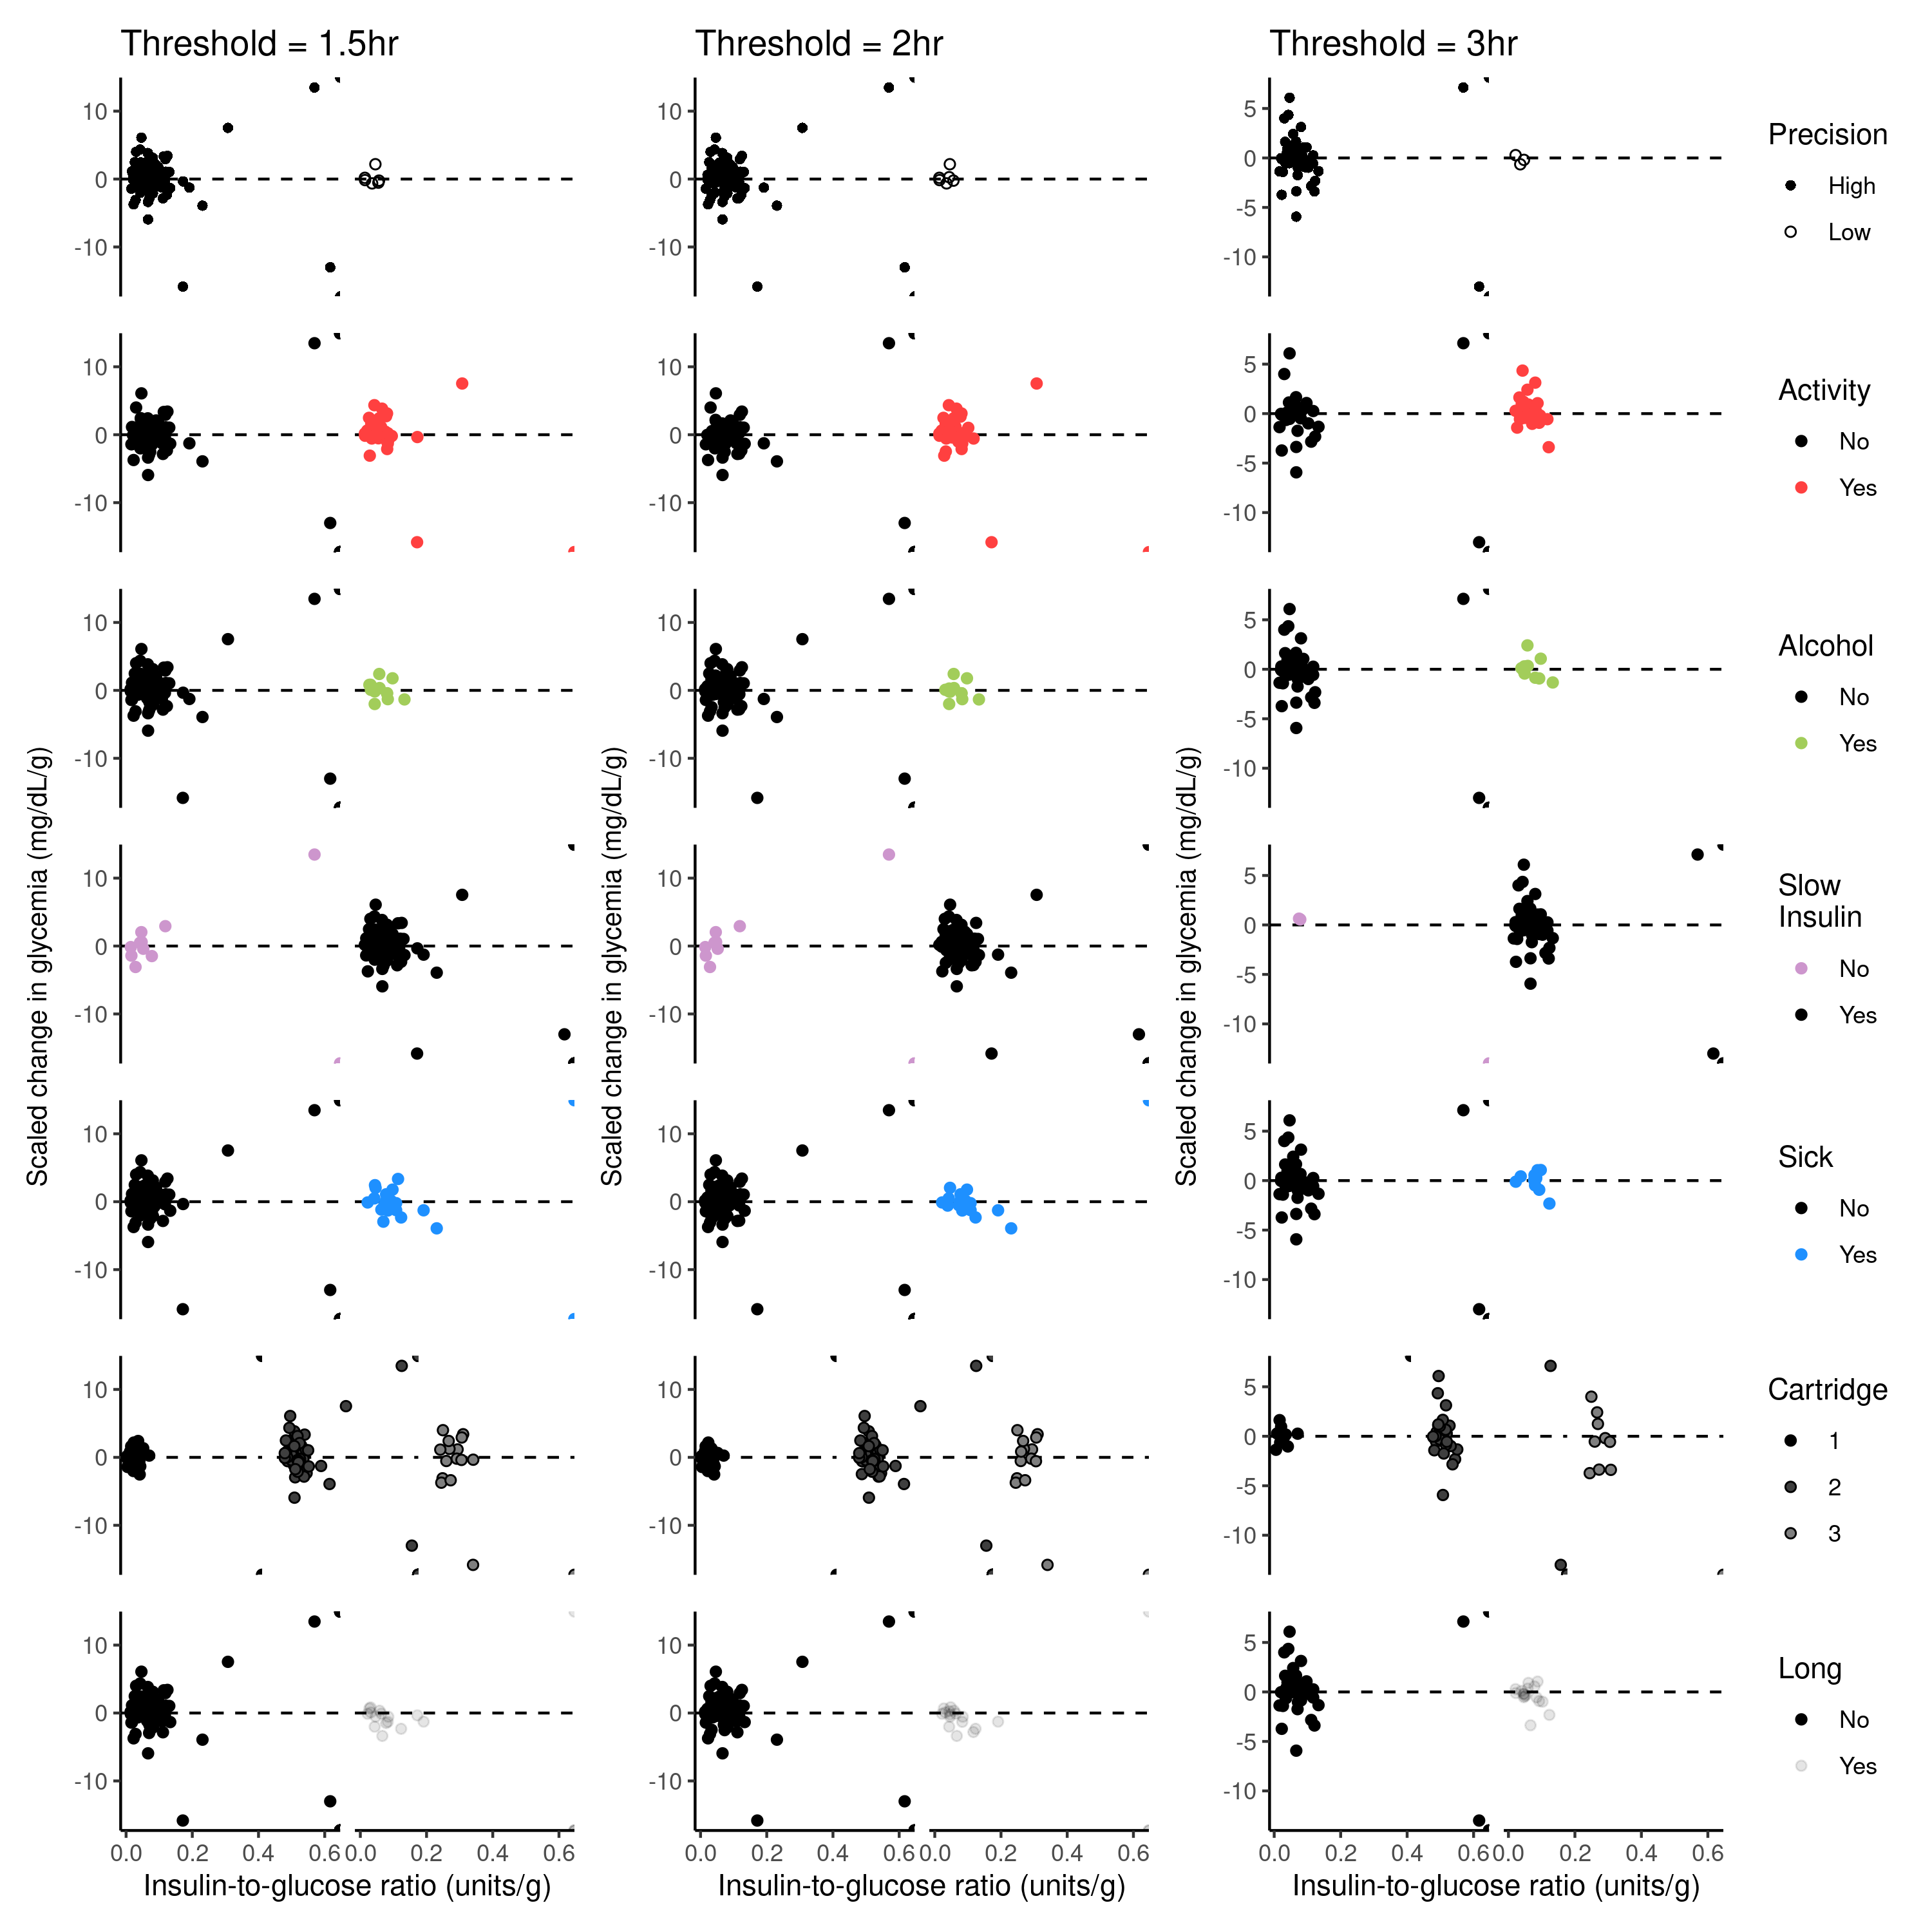
\includegraphics[width=\textwidth]{figures/overview_binary.png}
	\caption{Overview of the data split by various values of the confounding variables, and for three different time thresholds (see Methods). Precision, whether there was a low-precision glucose measurement; Activity, whether the total activity impact score was of 2 or more; Alcohol, whether the highest inebriation status was of 2 or more; Slow Insulin, whether slow insulin was having an effect; Cartridge, identifier for individual insulin cartridges; Long, whether the chunk was more than 500min long. Note the difference of scales when splitting by cartridge (because of three cartridges).}
	\label{fig:overview}
\end{figure}

\pagebreak

\begin{figure}[H]
	\centering
	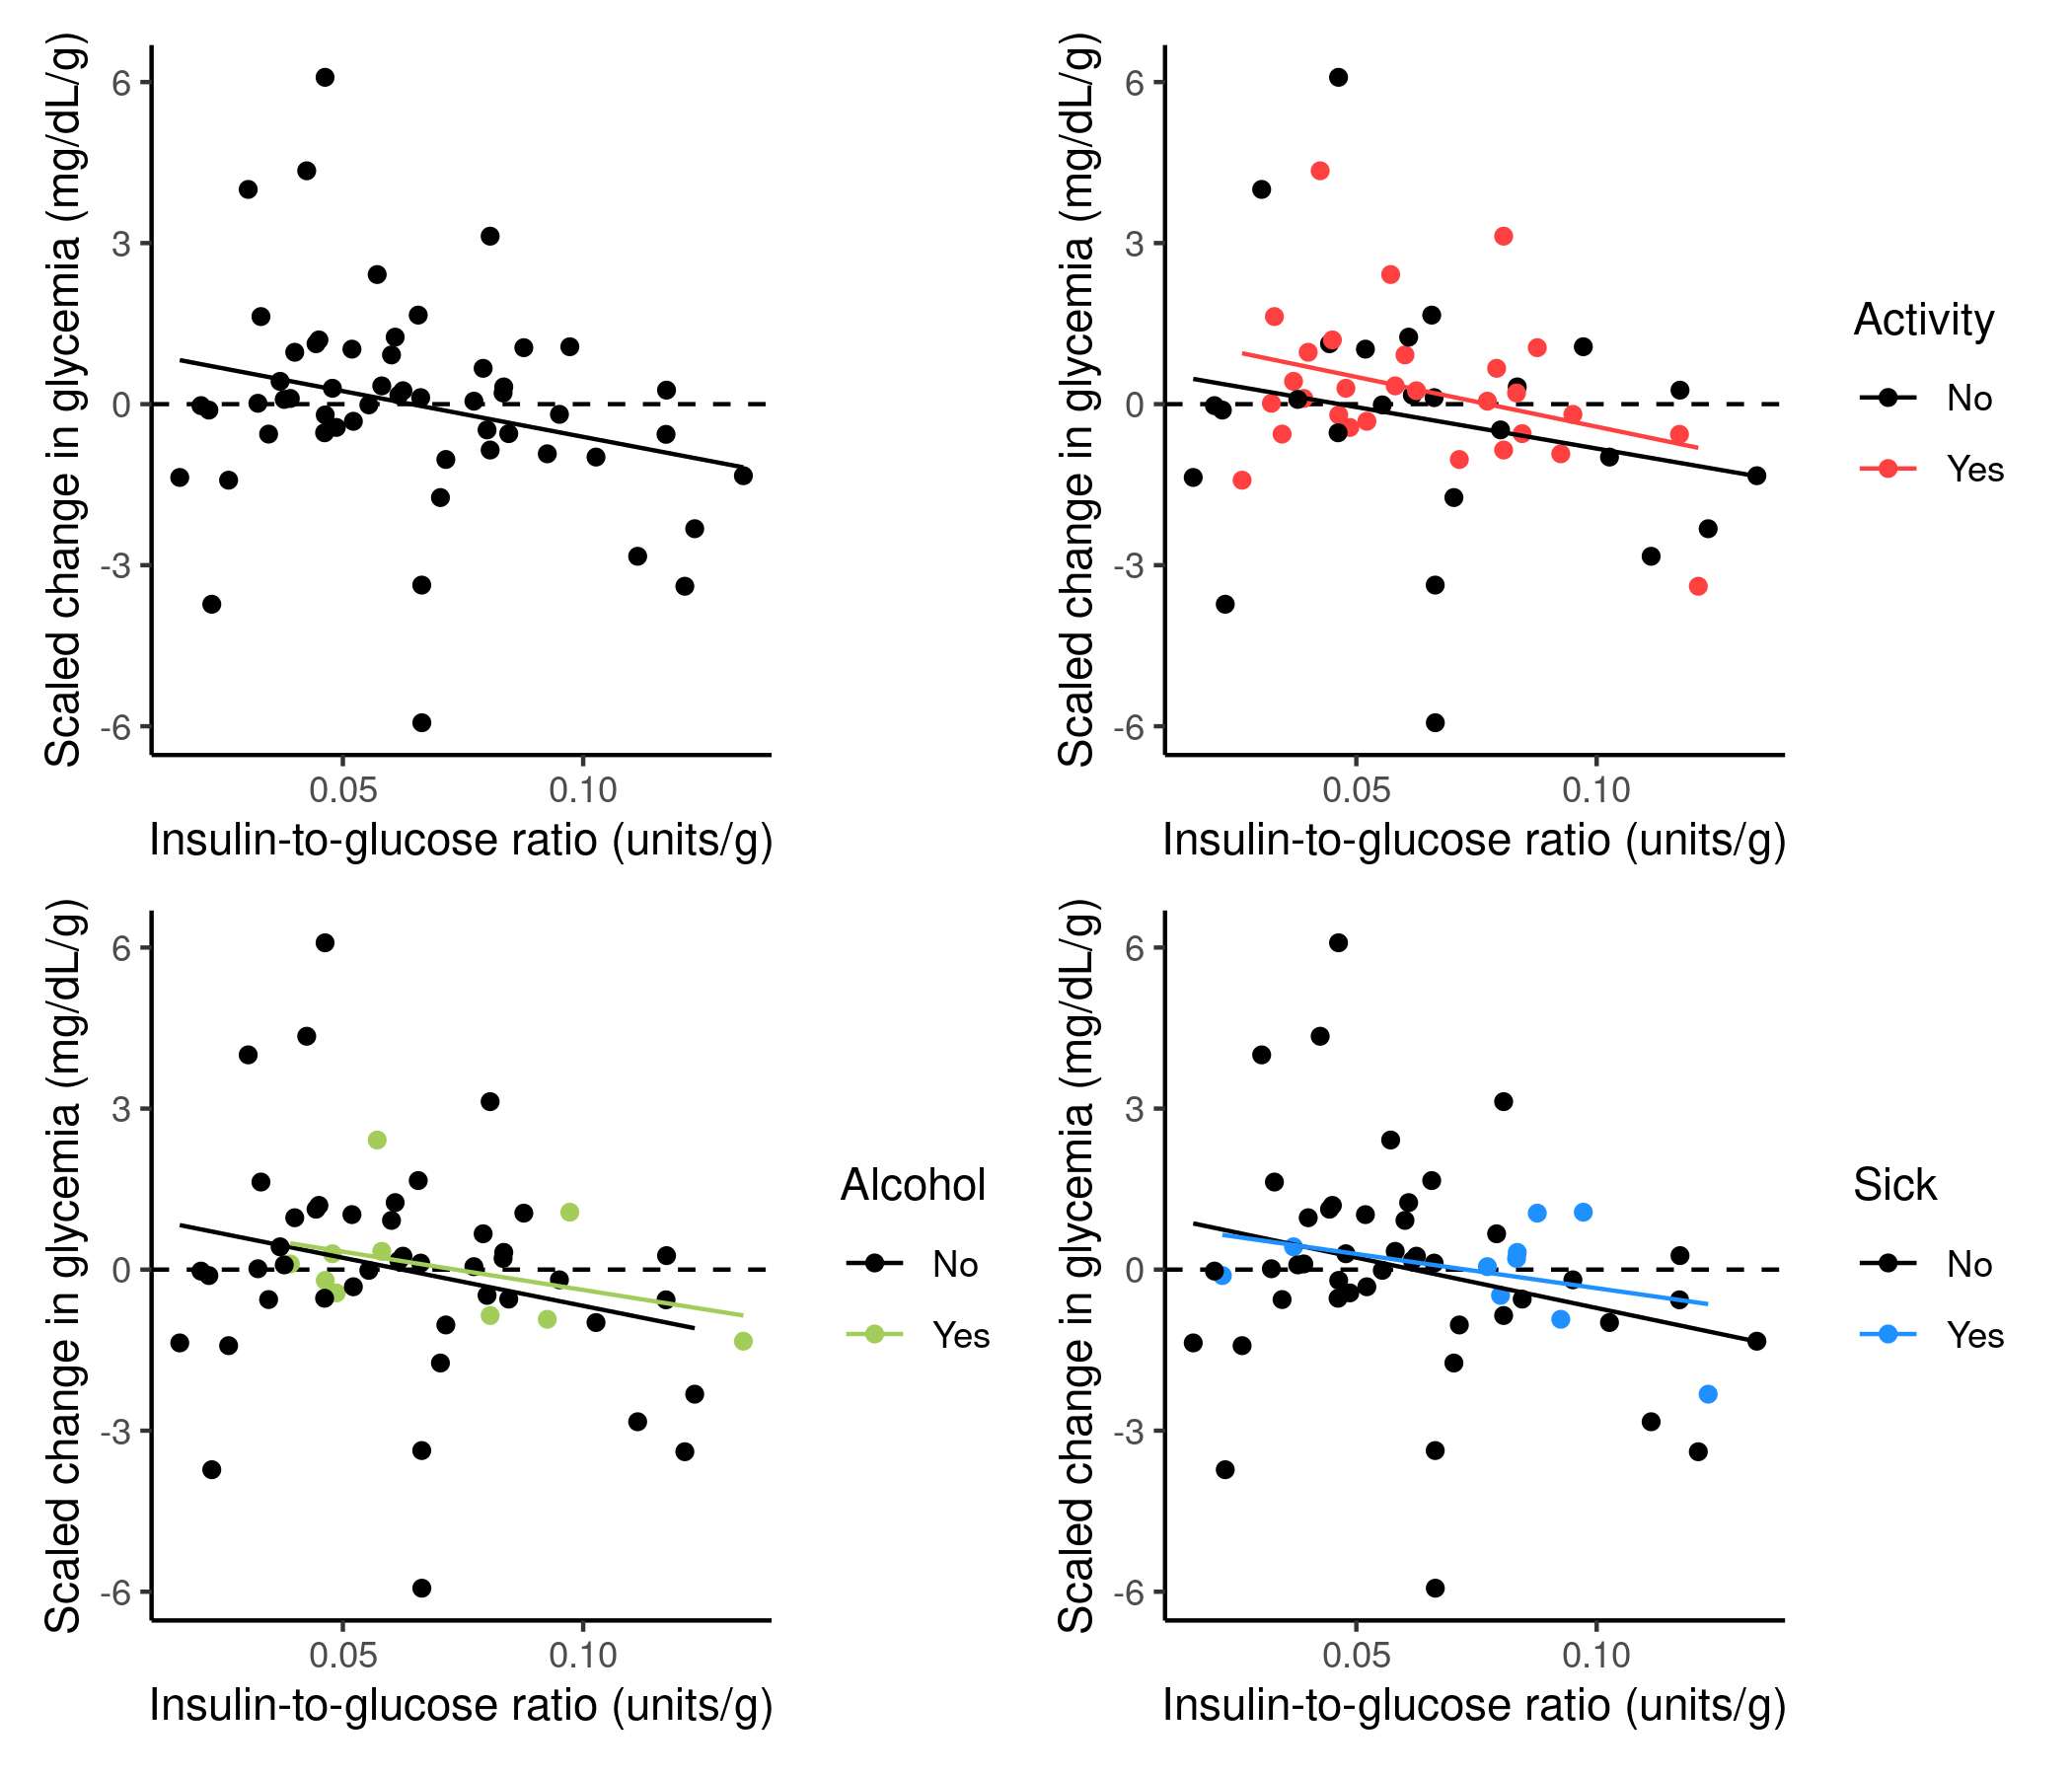
\includegraphics[width=\textwidth]{figures/separate_regressions_3_0.png}
	\caption{Four separate regression analyses of scaled change in glycemia against insulin-to-glucose ratio, either with no confounding variable (top left), or including activity (top right), alcohol (bottom left) or sickness (bottom right) as confounder. Those results are for a time threshold of 3 hours.}
	\label{fig:regressions}
\end{figure}